\documentclass[a4paper,11pt]{article}
\usepackage{CJKutf8}
\usepackage{listings}
\usepackage{graphics}
\DeclareGraphicsExtensions{.pdf,.png,.jpg}
\title{物联网工程2010级《操作系统》期中考试试卷}
\date{}
\date{2012年5月2日}

\begin{document}
\begin{CJK*}{UTF8}{gbsn}

\maketitle

\section{简答与计算(每题8分,共80分)}
\subsection{}
请用你自己的话简要说明什么是多道程序设计技术,以及为什么引入这种技术。
\\[1in]

\subsection{}
什么是CPU密集型进程?什么是I/O密集型进程?请针对这两类进程分别举两个实际例子。
\\[1in]

\subsection{}
请解释进程调度方法中,抢占式调度与非抢占式调度的具体含义以及二者各自的优缺点。
\\[1in]

\subsection{}
(a) 请指出进程概念与线程概念的本质区别。\\
(b) 为什么要引入多线程技术?
\\[1in]

\subsection{}
(a)  什么是程序访问的局部性原理?\\
(b)  什么是工作集(working set)?
\\[1in]

\subsection{}
在32位PC机上,采用分页技术(只利用一级页表),请回答: \\%如果虚拟内存系统按照4M大小对进程的虚拟地址空间进行分页,请回答:
(a) 如果每页大小为4M,则32位虚拟地址中需要多少位用于描述页内偏移(页内地址)? 多少位用于对页表进行索引?\\
(b) 如果每页大小为4K,且系统实际安装的物理内存大小为1G,则页表项中页框号这个字段至少需要多少个二进制位?
\\[1in]

\subsection{}
某进程在某一时刻的页表如下图所示,请计算该进程地址空间中虚拟地址8592所对应的物理地址的值。

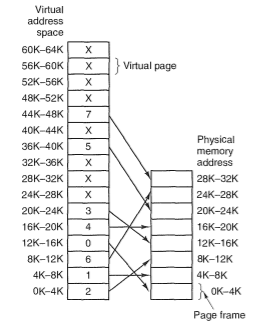
\includegraphics{vm.png}
\\[1in]

\newpage
\subsection{}
在生产者--消费者问题中,分别给出给出以下生产者和消费者程序代码,其中调用了操作系统提供的函数sleep和weakup.
请指出这段代码中存在的竞争条件.

%\lstset{language=C, frame=trbl}
%\lstinputlisting{prodcons.c}
\begin{verbatim}
#define N 100
int count = 0;
int buf[N];

void producer(void) {
    int item;

    while (1) {
        item = produce_item();
        if (count == N) sleep();
        insert_item(item);
        count += 1;
        if (count == 1) wakeup(consumer);
    }
}

void consumer(void) {
    int item;

    while (1) {
        if (count == 0) sleep();
        item = remove_item();
        count -= 1;
        if (count == N-1) wakeup(producer);
        consume_item();
    }
}
\end{verbatim}


\newpage
\subsection{}
阅读以下某机器汇编语言代码,并回答问题:

%\lstset{language=C, frame=trbl}
%\lstinputlisting{tsl.c}
\begin{verbatim}
enter_region:
    TSL REG, LOCK
    CMP REG, #0
    JNE enter_region
    RET

leave_region:
    MOVE LOCK, #0
    RET
\end{verbatim}
\begin{enumerate}
\item 简要说明以上代码中的TSL指令的功能。
\item 用这里定义的enter\_region和leave\_region可以实现进程互斥进入临界区,请说明原因。
\item 用上述方法实现互斥访问临界区的缺点是什么?
\item 在多核处理器上,上述方法实现互斥访问临界区有什么优点(注:考虑sleep和wakeup开销)?
\end{enumerate}

\newpage
\subsection{}
请从尽可能多的角度阐述图形用户界面与命令行界面各自优缺点。

\newpage
\section{Linux系统调用与C语言编程(每题10分,共20分)}

\subsection{}
以下程序的功能是比较两个文件是否相同(省略了头文件和必要的错误检测),但其中两行存在问题,请指出这两行的行号,并给出你对两处错误的修正结果。
%\lstset{language=C, frame=trbl}
%\lstinputlisting{prog2.c}
\begin{verbatim}
int main(int argc,char *argv[])
{
        int fd1,fd2;
        char buff1[1024], buff2[1024];
        int m,n;
        fd1=open(argv[1],O_RDONLY);
        fd2=open(argv[2],O_RDONLY);
        while(1)
        {       
                n=read(fd1,buff1,1024);   
                m=read(fd2,buff2,1024);
                if(strcmp(buff1,buff2)!=0 || n!=m )
                {
                        printf("not the same!\n");
                        return -1;           
                }
                if(n = 0)
                        break;          
        }
        printf("the two files are the same!\n");
        return 0;
}
\end{verbatim}

\newpage
\subsection{}
以下是一个简单的shell程序源代码,它可以执行不带参数和选项的命令(如不能执行用户命令则打印错误信息),并且可以支持
后台进程(用户输入命令以\&结尾),请在划线处补全程序。
\begin{verbatim}
#include <sys/wait.h>
#include <string.h>
#include <stdio.h>
#include <stdlib.h>
#include <unistd.h>
#define MAXLINE 4096

int main(void) {
        char    buf[MAXLINE];   
        pid_t   pid;
        int     status, background;

        printf("%% ");  
        while (fgets(buf, MAXLINE, stdin) != NULL) {
            background = 0;
            if (buf[strlen(buf) - 1] == '\n')
                buf[strlen(buf) - 1] = 0; /* replace newline with null */

            if (buf[strlen(buf) - 1] == '&') {
                ____________________;

                ____________________;
            }
            pid = fork();
            if (pid < 0) 
                exit(1);
            else if (pid == 0) {            /* child */
                execlp(buf, buf, (char *)0);

                ____________________;
                exit(127);
            }
            if ((pid = waitpid(pid, &status, background? WNOHANG : 0)) < 0)
                exit(2);
            printf("%% ");
        }
        exit(0);
}
\end{verbatim}


\end{CJK*}
\end{document}

